\documentclass[12pt]{article}
\usepackage{graphicx}
\usepackage{epstopdf}
\usepackage[backend=bibtex,style=alphabetic,natbib=true]{biblatex} % (which resembles APA)
\addbibresource{kcorebip.bib} % The filename of the bibliography

\title{Using the kcorebip package}
\author{Javier Garcia-Algarra}

\begin{document}

\flushbottom
\maketitle

\thispagestyle{empty}

\section*{Introduction}

This package performs the \textit{k-core decomposition} analysis of a bipartite graph and provides two new kinds of plot: \textit{polar} and \textit{ziggurat}. It works for
any kind of bipartite network, but we developed it to study ecological mutualistic communities, so we use terminology and examples of that research field.

\section*{Decomposition and definition of k-magnitudes}
\label{K-magnitudes}

The \textit{k-decomposition} is an iterative algorithm that prunes links of nodes with degree equal or less than $k$. The process starts pruning nodes with $k=1$ until all the resting nodes have two or more links. Then it continues with $k=2$, and so on. After performing the \textit{k-decomposition}, each species belongs to one of the \textit{k-shells}. The highest value of \textit{k}, i.e $ks_{max}$, corresponds to the innermost \textit{core} $ks_{max}\equiv C^{A,B}$. For each \textit{k-shell} there are two subsets, one per guild ($A$ and $B$), that we call $K^{A}_{j}, K^{B}_{j}$ where $j$ is the \textit{k-shell} index.

In order to quantify the distance from a node to the innermost shell of the partner guild, we calculate the average of the shortest paths to all the nodes in that set. We define the \textit{$k_{radius}$} of node $m$ of class $A$ as the average distance to the species of $C^B$:

\begin{equation}
\displaystyle
k^A_{radius}(m) = \frac{1}{\mid C^{B} \mid}\sum\limits_{j \in C^{B}} dist_{mj}  \qquad   m \in A
\label{kradius}
\end{equation}

\noindent where $dist_{mj}$ is the shortest path from species $m$ to each of the $j$ species that belong to the set $C^B$. The same definition is valid for species of the guild $B$ computing the average distance to $C^A$. The minimum possible radius value is $1$ for one node of the maximum shell directly linked to each one of the maximum shell set of the opposite guild.

\begin{figure}[h!]
\centering
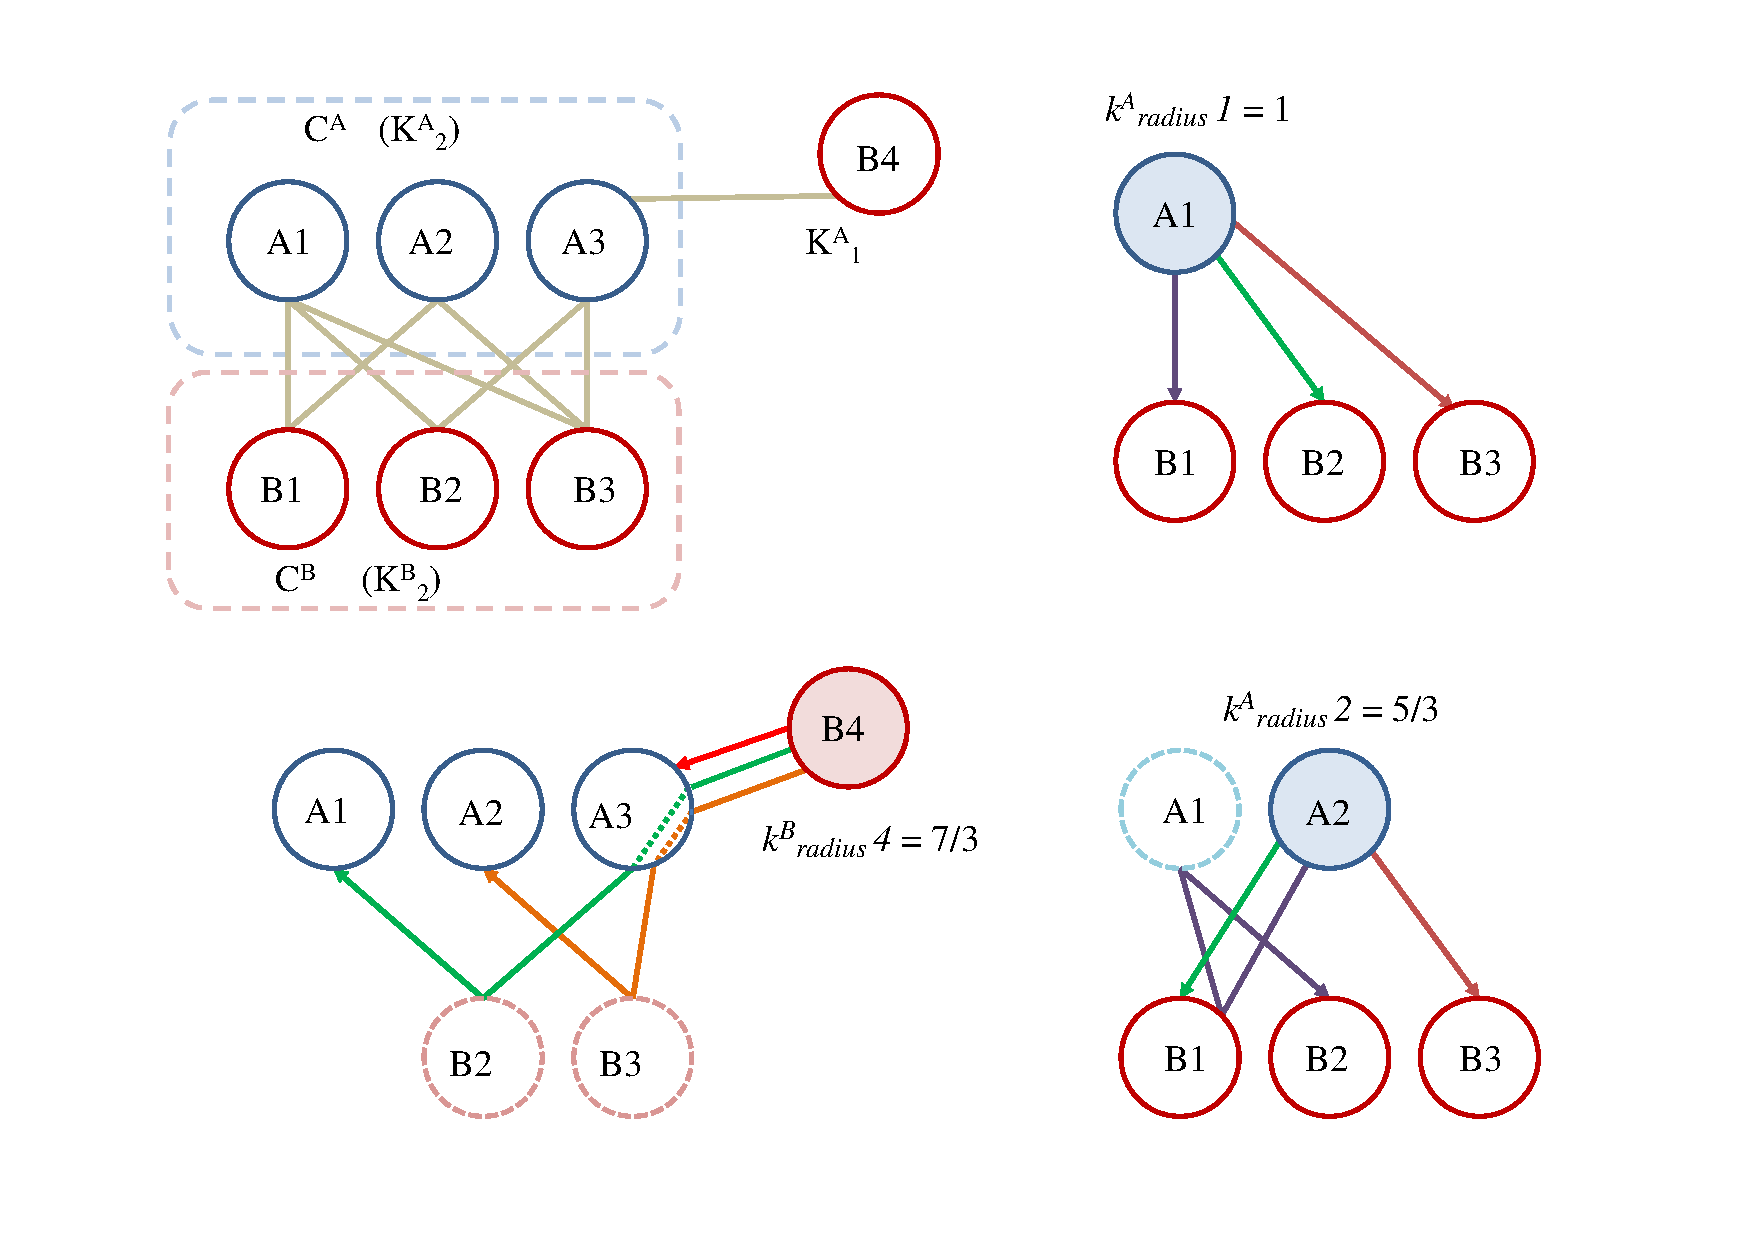
\includegraphics[scale=0.4]{red_example.pdf}
\caption {Examples of \textit{$k_{radius}$} in a fictional network.}
\label{fig:red_example}
\end{figure}

Figure \ref{fig:red_example} is a very simple fictional network, with only seven nodes. The upper left graph shows network structure. In the upper right figure, species $A1$ belongs to $C^{A}$.  The distance to each of the nodes of $C^{B}$ is $1$, so its \textit{$k^A_{radius1}(1)$} is $1$. In the bottom right figure, node  $A2$ also belongs to $C^{A}$ but there is not any direct link with $B2$, so the distance between them is $3$ and \textit{$k_{radius}(2)$} is $\frac{5}{3}$. In the bottom left figure, node $B4$ is not part of $C^{B}$, and as may be expected, the value of its \textit{$k_{radius}$} is higher. 

A global value can be defined averaging this magnitude across network:

\begin{equation}
\displaystyle
\overline {k}_{radius} = \frac{1}{\mid A \cup B \mid}\sum\limits_{l \in A \cup B} k_{radius}l
\label{avgkradius}
\end{equation}

In our example network of Figure \ref{fig:red_example}, the value is $11/7$. 

${k}_{radius}$ is a useful magnitude \emph{to measure nestedness} but it not a good measure of centrality. For instance, its value for an isolated specialist linked to the maximum core is low. \emph{To attend this necessity,} we define a second \textit{k-magnitude}, the ${k}_{degree}$:

\begin{equation}
\displaystyle
k^A_{degree}m = \sum\limits_{j} \frac{a_{mj} }{k_{radius}j}  \quad   m \in A, \forall j \in B
\label{kdegree}
\end{equation}

\noindent where $a_{mj}$ is the element of the interaction matrix that represents the link. So the $k_{degree}m$ is the sum of the inverse of $k_{radius}$ for each node linked to $m$. A node of the innermost shell will have a high degree, whereas specialists have only one or two links and so a low $k_{degree}$. In the example of Figure \ref{fig:red_example}, this magnitude is $1+3/5+3/5 = 11/5$ for node $B3$, while only $3/7$ for node $B4$. 


\subsection*{The Polar Plot}
\label{visualizations}

We have designed two new kind of  visualizations for mutualistic networks, using $k_{radius}$ and $k_{degree}$. We call the first one \textit{Polar Plot}. Its purpose is showing species centrality and having a quick overview of network distribution. It was inspired by the \textit{fingerprint-like} graph, developed by Alvarez-Hamelin \textit{et al.} \cite{alvarez:2005k} to plot very large \textit{k-decomposed} networks.

Species are depicted with their centers located at $k_{radius}$. Angles are assigned at random by the visualization algorithm to reduce overlapping, with the condition that each guild lies inside one of the half planes. Shape underlines the guild separation. The area of each node is proportional to its $k_{degree}$ and the color represents the $k_{shell}$. This visualization does not include links. The user may choose adding the histograms of \textit{k-magnitudes}, a handy option because they convey a wealth of structural information.

%Figure \ref{fig:red_example} is a real mid size network. A reduced number of nodes have a high $k_{degree}$, while most species are peripheral. 

Polar graph is specially useful when comparing different networks side by side, even if they are of very different sizes. In Figure \ref{fig:polar_diagrams}, we have picked thr
\textit{Ziggurat diagram} is the second type of visualization, created from scratch. The idea behind it is splitting species in sets by their $k$-$shells$. Each of these groups are represented as small ziggurats. The maximum $k$-$shell$ is located on the left side, the other ones are arranged following an almond distribution. Species of this shell are ordered by their $k_{degree}$ with the higher one leftmost. Areas do not convey meaning, their height decreases just by convenience of visualization. 

Nodes of $1$-$shell$ are scattered around the ziggurats. When multiple species of this shell are connected to the same node of any of the ziggurats they are clustered to reduce the number of lines. For instance, in Figure \ref{fig:ziggurat} plants species $22, 30$ and $33$ are specialists linked to the generalist disperser $3$. With this organization, we get a clear view of structure and interconnections. The almond shape leaves a wide space in the center of the graph to depict the links and they do not overcross the boxes of the different species.





\begin{figure}[h!]
\centering
\includegraphics[scale=0.4]{ALL_SD_004.eps}
\caption {Ziggurat graph of an avian frugivore community in Puerto Rico with 54 species and 95 links\cite{carlo:2003avian}. Below, the classical bipartite graph of the same network.}
\label{fig:ziggurat}
\end{figure}

The network of Figure \ref{fig:ziggurat} has 95 links. It is still possible to see details in the bipartite graph, as nodes highly connected. With a higher number of interactions it becomes a \textit{spaghetti dish} mess. The ziggurat gives a clear glimpse of the internal organization with four shells and a tiny external layer. Patterns may be visually discovered, for instance the low number of links between species of lower shells, or the relative low centrality of disperser species number $2$ that appears leftmost in the bipartite graph. 


\printbibliography[heading=bibintoc]

\end{document}
